\documentclass[a4paper,10pt]{article}

\usepackage{ifpdf}
\usepackage[spanish]{babel}
\usepackage{ucs}
\usepackage[utf8x]{inputenc}
\PrerenderUnicode{áéíóúñ}
\usepackage[T1]{fontenc}
\usepackage{charter}

\addto\captionsspanish{\def\tablename{Tabla}}

\ifpdf
	\usepackage[pdftex]{color,graphicx}
	\usepackage[pdftex]{hyperref}
\else
	\usepackage[dvips]{color,graphicx}
	\usepackage[dvips]{hyperref}
\fi
\usepackage{wrapfig}
\usepackage{fancyvrb}
\DefineVerbatimEnvironment{SmallVerbatim}{Verbatim}{fontsize=\scriptsize, tabsize=4}
\DefineVerbatimEnvironment{SmallVerbatimNum}{Verbatim}{numbers=left, fontsize=\scriptsize, tabsize=4}

% Cabezal y pie de página
\usepackage{fancyhdr}
\pagestyle{fancy}
\renewcommand{\sectionmark}[1]{\markright{\thesection\ #1}}
\fancyhf{}
\fancyhead[L]{\rightmark}
\fancyhead[R]{\thepage}
\fancyfoot[L]{}
\fancyfoot[R]{}
\renewcommand{\headrulewidth}{0.5pt}
\renewcommand{\footrulewidth}{0pt}
\addtolength{\headheight}{0.5pt} % Hacer espacio para la linea del cabezal
\fancypagestyle{plain}{% Sacar cabezales en plain pages
	\fancyhead{}
	\renewcommand{\headrulewidth}{0pt}
}

\hypersetup{colorlinks=true}
\hypersetup{citecolor=blue}
\hypersetup{filecolor=black}
\hypersetup{linkcolor=blue}
\hypersetup{urlcolor=blue}
\hypersetup{pdfauthor={Gastón Simone}}
\hypersetup{pdftitle={Versión inicial de una biblioteca para la enseñanza de álgebra lineal numérica}}

\title{Versión inicial de una biblioteca para la enseñanza de álgebra lineal numérica}
\author{Gastón Simone, Pablo Ezzatti\vspace{0.5cm} \\ Instituto de Computación\\ Facultad de Ingeniería, Universidad de la República\\ J. Herrera y Reissig 565, Montevideo, Uruguay\\ \url{gaston.simone@gmail.com}\\ \url{pezzatti@fing.edu.uy}}
\date{Junio 2008}

\begin{document}

\maketitle

\textbf{Palabras claves:} Álgebra Lineal Numérica, C, Algoritmos.

\begin{abstract}
%Durante la edición 2008 del curso de Álgebra Lineal Numérica, dictado por el Instituto de Computación, se realizó la implementación de una biblioteca de utilidades para el trabajo con sistemas lineales dispersos, en calidad de proyecto de fin de curso. 
La resolución de una gran cantidad de modelos presentes en la computación científica se basan en la solución de problemas del álgebra lineal numérica (ALN). 
Esta situación ha motivado fuertemente el desarrollo del área.
En contraposición al importante desarrollo se ha incrementado en forma abrupta la complejidad de las estrategias de resolución utilizadas, dificultando la comprensión por parte de los alumnos de los algoritmos utilizados.

En este contexto la propuesta se centra en el desarrollo de una biblioteca de ALN de carácter didáctico. 
%La implementación de la biblioteca se hizo pensando en todo momento en su uso didáctico.
Por esta razón, la documentación es vasta y el código fue escrito pensando en su fácil lectura. Las rutinas implementadas son eficientes desde el punto de vista algorítmico. 
Pero determinadas mejoras de desempeño, propias de la implementación, fueron descartadas para mantener la legibilidad del código.

Este documento presenta el diseño, las funcionalidades y la implementa-ción realizada.
Se describe también la documentación técnica que acompaña a la implementación, la cual es de utilidad para el estudio. 
Finalmente se mencionan conclusiones y se describen posibles trabajos futuros sobre la herramienta construida.
\end{abstract}

\newpage

%\tableofcontents

\section{Introducción}

La resolución de una  gran cantidad de problemas presentes en la computación científica, en particular aquellos que utilizan modelados matemáticos para simular procesos físicos, necesitan como parte fundamental en cuanto a tiempos de cómputo la resolución de problemas de álgebra lineal numérica (ALN).
Esta realidad ha motivado a que muchos grupos de investigación a nivel mundial centren su trabajo en el desarrollo del área. 
Esta situación se puede verificar observando por un lado la gran cantidad de bibliotecas desarrolladas en los últimos años y por otro constatando la importante disminución en los tiempos de ejecución necesarios para la resolución de grandes sistemas lineales.
 
En contraposición con el gran desarrollo en cuanto a los niveles de eficiencia en los métodos de resolución logrados se ha incrementado en forma notoria la complejidad de los algoritmos. 
Entre otras cosas se ha perdido en  la legibilidad de los programas, en lo intuitivo de las técnicas, etc.
%Utilizando técnicas cada vez más complejas y buscando la optimización 

Estas dificultades en la comprensión de los algoritmos utilizados en el área obstaculizan el acercamiento por parte de los alumnos de grado a las distintas problemáticas y las estrategias de resolución. 
Teniendo como consecuencias directas, por un lado la disminución de profesionales con capacidades en los temas de ALN y por otro lado el alejamiento de los jóvenes investigadores en épocas tempranas del área.

Este trabajo presenta una propuesta de biblioteca de ALN, la cual busca facilitar la comprensión de los algoritmos involucrados en el tratamiento de matrices dispersas.
La intensión es que la biblioteca posea un carácter didáctico, resignando en muchas ocasiones la eficiencia en los algoritmos para priorizar la facilidad de comprensión.

Los requisitos planeados en el párrafo anterior condicionaron en la etapa de diseño que la arquitectura de la biblioteca permitiera diversas extensiones.
Previendo en un futuro cercano poder trabajar con otros formatos de matrices dispersas, incluir nuevos métodos o incluir estrategias de programación en paralelo. 
También se tomó especial énfasis en la documentación de la biblioteca.

% La primer versión de la biblioteca, 
%Parte de e
Este documento describe la primera versión de la biblioteca, que se denomina BAL (por el -acrónimo- Biblioteca de Álgebra Lineal).
También se presentan posibles usos de la biblioteca en la enseñanza del álgebra lineal numérica. 
Es importante establecer que el trabajo es el puntapié inicial de un proyecto más ambicioso. 
Esperando desarrollar más material que sirva para potenciar el trabajo de enseñanza e investigación en temas referentes al ALN.

El documento está estructurado de la siguiente forma. La sección 2 brinda un detalle de las funcionalidades actualmente disponibles en BAL. 
La sección 3 brinda una reseña de la estructura interna de BAL, cómo fueron agrupadas las distintas funcionalidades dentro de la biblioteca.
En la sección 4 se describen componentes adicionales que acompañan la implementación de la biblioteca. 
La sección 5 describe los pasos necesarios para utilizar BAL.
Luego, la sección menciona algunas ideas para el uso de BAL como una herramienta didáctica.  
Finalmente, la sección 7 menciona las conclusiones sobre el trabajo realizado y describe el trabajo futuro a partir de la situación actual.

%La aprobación del curso 2008 de la asignatura opcional \emph{Álgebra Lineal Numérica} del Instituto de Computación (InCo) constó de dos instancias.
%La primera fue la exposición de un tema por parte del estudiante, en una de las clases dictadas durante el curso.
%La segunda constó de la elaboración de un trabajo final, en el que se aplicara lo aprendido en el curso, o bien se profundizara el estudio en algún tema en particular. Los trabajos finales eran sugeridos por los docentes o propuestos por los alumnos.

%Uno de los trabajos sugeridos fue la elaboración de una biblioteca para matrices dispersas, en la que se pudieran manejar varios formatos y que además implementara distintos algoritmos, como factorización de matrices, aprovechando los beneficios de los formatos dispersos. Esta propuesta fue tomada por Gastón Simone, quien, bajo la tutoría del profesor Pablo Ezzatti del InCo, llevó a cabo el proyecto.

%La primer versión de la biblioteca, llamada \emph{BAL} (por \emph{Biblioteca de Álgebra Lineal}), es la que correspondió a la entrega final del curso y fue llamada \emph{BAL 2008}.
%Parte de este documento describe la primera versión de la biblioteca, junto con su posible uso en la enseñanza del Álgebra lineal.

%El documento está estructurado de la siguiente forma. La sección \ref{sec_funcionalidad} brinda un detalle de las funcionalidades actualmente disponibles en BAL. La sección \ref{sec_estructura} brinda una reseña de la estructura interna de BAL, cómo fueron agrupadas las distintas funcionalidades dentro de la biblioteca. En la sección \ref{sec_componentes} se describen componentes adicionales que acompañan la implementación de la biblioteca.
%La sección \ref{sec_uso} describe los pasos necesarios para utilizar BAL. Luego, la sección \ref{sec_ens} menciona algunas ideas para el uso de BAL como una herramienta didáctica. Finalmente, la sección \ref{sec_futuro} menciona las conclusiones sobre el trabajo realizado y describe el trabajo futuro a partir de la situación actual.

\section{Funcionalidades actuales de la biblioteca}
\label{sec_funcionalidad}
A continuación se detallan las distintas funcionalidades disponibles actualmente en BAL.
\begin{enumerate}
 \item Cargas de datos desde archivo
 \begin{enumerate}
  \item Leer definiciones de matrices dispersas en el mismo formato utilizado por MatLab \cite{matlab}.
  \item \label{leer_simple} Leer definiciones de matrices en un formato para matrices dispersas por coordenadas. %\footnote{Vea el primer formato definido en la sección 5.1 de Stewart~\cite{stewart}}.
 \end{enumerate}
 \item Formatos de matrices dispersas manejados \cite{dongarra}
 \begin{enumerate}
  \item Simple por coordenadas.
  \item Empaquetado por columnas (CSC).
  \item Comprimido por diagonales (CDS).
 \end{enumerate}
 \item Impresión de estructuras de datos
 \begin{enumerate}
  \item Impresión de detalle de estructuras en memoria, para todos los formatos de matrices dispersas soportados.
  \item Impresión de matrices en memoria a formato matlab, para formatos CSC y CDS.
  \item Impresión de matrices en memoria en formato simple al mismo formato esperado en \ref{leer_simple}.
 \end{enumerate}
 \item Funciones de conversión entre formatos dispersos
 \item Funciones de soporte
 \begin{enumerate}
  \item Liberación de memoria utilizada en estructuras creadas con BAL.
 \end{enumerate}
 \item Algoritmos
 \begin{enumerate}
  \item Recorrer por filas una matriz empaquetada por columnas en forma eficiente.
  \item Producto matriz-vector optimizado para matrices simétricas en formato CSC.
  \item Producto matriz-vector optimizado para matrices en formato CDS.
  \item Producto matriz-matriz optimizado para matrices en formato CDS.
  \item Cálculo del árbol de eliminación \cite{Liu} de una matriz en formato CSC.
  \item Factorización simbólica de una matriz en formato CSC.
  \item Factorización de Cholesky de una matriz en formato CSC.
  \item Resolución de un sistema lineal triangular, representado con una matriz en formato CSC.
 \end{enumerate}
\end{enumerate}
La lista completa de las funcionalidades se pueden obtener en la documentación técnica \cite{bal_tecnica}.

\section{Estructura}
\label{sec_estructura}
A continuación se menciona cómo están distribuidas las distintas funcionalidades de BAL dentro de sus archivos fuente. Conjuntamente se brindan algunos detalles técnicos de la implementación de las distintas funcionalidades.

\begin{wrapfigure}{r}{0.25\textwidth}
  \vspace{-20pt}
  \begin{center}
	\ifpdf
		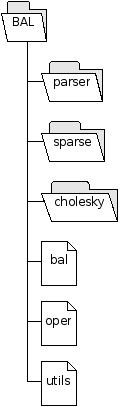
\includegraphics[height=5cm]{img/estructura.png}
	\else
		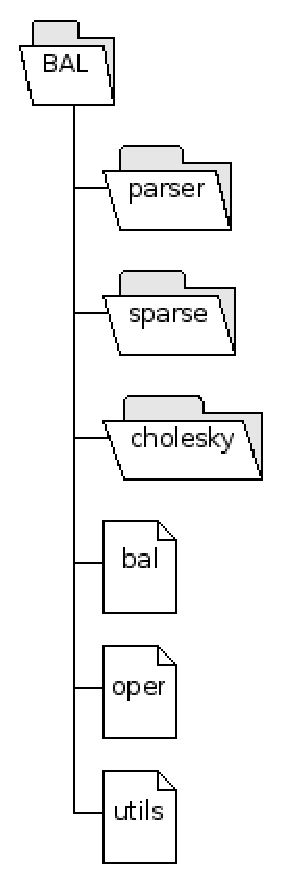
\includegraphics[height=5cm]{img/estructura.eps}
	\fi
  \end{center}
  \vspace{-20pt}
  \caption{Estructura de directorios de BAL}
  \vspace{-40pt}
\end{wrapfigure}
El directorio raíz de BAL contiene (además de archivos de soporte como el \texttt{makefile} y el archivo de configuración de la documentación autogenerada) los módulos llamados \texttt{bal}, \texttt{oper} y \texttt{utils}. El módulo \texttt{bal} define un medio de acceso a todas las funcionalidades de BAL de forma homogénea. De este modo, un programa cliente que desee utilizar BAL solo debe agregar la instrucción de preprocesador
\begin{SmallVerbatim}
#include <bal.h>
\end{SmallVerbatim}
y ya estará en condiciones de utilizar todas las funcionalidades de BAL. Por otra parte, el módulo \texttt{utils} contiene funciones de utilidad general que son utilizadas a lo largo de todo el código de BAL. El módulo \texttt{oper} implementa los algoritmos de operaciones básicas, del tipo matriz-vector y matriz-matriz.

El directorio \texttt{parser} de BAL contiene  la implementación del parser de definición de matrices en formato matlab~\cite{matlab}. Este parser es implementado mediante código autogenerado utilizando las herramientas \texttt{GNU bison}~\cite{bison} y \texttt{flex}~\cite{flex}. El archivo \texttt{matriz\_scanner.lex} contiene la definición del analizador lexicográfico generado por \texttt{flex}, mientras que el archivo \texttt{matriz\_parser.y} define una gramática libre de contexto, junto con el código necesario para que \texttt{bison} genere el parser buscado.

El directorio \texttt{sparse} contiene las definiciones de las estructuras de datos para matrices dispersas, así como también la implementación de las funciones de conversión entre estas representaciones.
El módulo \texttt{sp\_coord} define la estructura simple por coordenadas, así como también implementa las herramientas básicas para trabajar con la estructura. De la misma forma, los módulos \texttt{sp\_packcol} y \texttt{sp\_cds} lo hacen para los formatos CSC y CDS.

Finalmente, el directorio \texttt{cholesky} contiene la implementación de las distintas rutinas que permiten la resolución de un sistema de ecuaciones mediante la factorización de Cholesky~\cite{duff}. Esta resolución se entiende como la ejecución de las siguientes etapas \cite{george}:
\begin{enumerate}
 \item Reordenamiento.
 \item Cálculo del árbol de eliminación.
 \item Factorización simbólica.
 \item Factorización numérica.
 \item Resolución de sistemas triangulares.
\end{enumerate}

\pagebreak
El módulo \texttt{cholesky} implementa todas las etapas de la resolución, menos la etapa de reordenamiento, para la cual aun no se cuenta con la implementación de un algoritmo. Pero la biblioteca ya dispone de la estructura necesaria como para agregar tal etapa fácilmente. Esto se hará mediante la extensión del módulo \texttt{reordenamiento}.

La gran mayoría de la implementación de este método de resolución está basado en el paper de Stewart~\cite{stewart}. 

%Durante su estudio e implementación se encontraron pequeños detalles en los pseudo-códigos presentados en el artículo, los cuales fueron corregidos en BAL. Tales cambios están bien señalados en el código y en la documentación técnica que acompaña a BAL. Esto hace que combinar la lectura del paper junto con el estudio y uso de BAL logre un valor agregado para el estudiante.

\section{Componentes adicionales}
\label{sec_componentes}
\subsection{Documentación técnica}
La biblioteca viene acompañada de un conjunto de documentación técnica que describe los detalles de las funcionalidades implementadas, describe los algoritmos y explica las estructuras de datos definidas.

Esta documentación fue creada con la herramienta Doxygen~\cite{doxygen}. La misma es generada en los formatos HTML y PDF, siendo el primero el recomendado debido a la facilidad de navegación que presenta.
 La misma documentación técnica explica cómo ésta es generada.

\subsection{Juego de pruebas}
Junto con la implementación de la biblioteca, se escribió un conjunto de programas que sirven no solo para verificar la correctitud de BAL, sino también como ejemplo de su uso.

Estos tests se encuentran en el directorio \texttt{bal\_test}. Cada prueba es un programa \texttt{C} diferente que se limita a probar una funcionalidad particular de BAL. El nombre del archivo \texttt{.c} da idea de lo que se pretende probar.

El juego de pruebas tiene su propio \texttt{makefile} para la fácil compilación. Pero más aun, el directorio de pruebas contiene un script llamado \texttt{run\_tests.sh} para la ejecución fácil de las pruebas. Este script, primero ejecuta el comando \texttt{make} para cerciorar que los tests han sido compilados. Luego busca aquellos tests que fueron compilados correctamente y los ejecuta. Para cada test ejecutado, redireccióna su salida estándar a un archivo de extensión \texttt{.out} y su salida de errores a una archivo de extensión \texttt{.error}. El prefijo de ambos archivos es el nombre del ejecutable del test\footnote{Nota: Para que este mecanismo funcione es importante que todos los ejecutables de las pruebas tengan sufijo \texttt{\_test}.}.

Al finalizar, el script muestra en pantalla una lista de aquellos tests que generaron algún tipo de salida  de errores. De este modo es fácil localizar cuáles tests fallaron.

\section{Uso de la biblioteca}
\label{sec_uso}
La biblioteca fue construida y probada bajo un ambiente UNIX utilizando el lenguaje \texttt{C}. Sin embargo, dada la portabilidad del lenguaje, no debería ser difícil conseguir que la misma funcione en otras plataformas.

La biblioteca se construye como un paquete precompilado. Una vez construida, un programa cliente puede utilizarla enlazando dicho paquete junto con su código, en tiempo de compilación.
El archivo \texttt{makefile} principal contiene una secuencia de pasos para instalar la biblioteca de forma permanente en el sistema. De este modo se facilita su utilización. Este modo de instalación también genera una copia de la documentación técnica dentro del sistema, para que esté disponible para todo usuario del mismo junto con la biblioteca.

La documentación técnica detalla todos los pasos necesarios para crear una aplicación que utilice la biblioteca, incluyendo compilación e instalación de la biblioteca, así como también compilación de un programa externo que haga uso de la misma.

\section{Utilización en la enseñanza del Álgebra Lineal Numérica}
\label{sec_ens}
Como ya fue mencionado, uno de los objetivos de este trabajo fue construir una herramienta que sirva para el estudio del álgebra lineal numérica. La biblioteca construida es el primer paso en este cometido. Con la versión 1.0.0 de BAL se cuenta con suficientes herramientas como para complementar el material teórico y práctico de algunos temas tratados durante un curso básico de ALN, como por ejemplo formatos de matrices dispersas, algoritmos eficientes con matrices dispersas, algoritmos de reordenamiento, factorización simbólica y factorización numérica.

Se pueden construir aplicaciones basadas en BAL que permitan realizar ejemplos durante una clase. Se pueden realizar comparaciones de performance entre BAL y otras herramientas, como por ejemplo matlab.
Los alumnos pueden hacer sus propias pruebas con la biblioteca e incluso extenderla. 
También se puede tomar la extensión de la biblioteca como trabajo importante en la comprensión de los algoritmos.

También es importante destacar que la documentación técnica que acompaña la implementación aporta el soporte necesario para el estudio de los algoritmos implementados y las estructuras de datos utilizados.
 La forma en la que es presentada la documentación junto con el código al que corresponde cada sección beneficia su lectura.

\section{Conclusiones y trabajo futuro}
\label{sec_futuro}
La biblioteca es un trabajo en progreso. Esta versión fue un paso inicial en la construcción de una herramienta de enseñanza, de práctica y una fuente de conocimiento en la rama del álgebra lineal numérica.
La disponibilidad de un conjunto de implementaciones fuertemente documentadas de distintos algoritmos básicos y otros más complejos es de gran valor para toda persona relacionada con la materia. El material desarrollado se puede obtener en \cite{bal_sitio}.\\

El trabajo futuro, en lo que refiere a la extensión de la biblioteca, tiene varios aspectos a ser considerados, a saber:
\begin{itemize}
 \item Se puede agregar soporte para más plataformas, en particular la plataforma Windows. Dado que gran parte de las instalaciones disponibles en facultad proveen esta plataforma, esto facilitaría el uso de la herramienta por parte de los alumnos.
 \item La biblioteca puede ser extendida para que determinados algoritmos produzcan salida que muestre la evolución de la ejecución de los mismos. Esto puede ser de gran ayuda a la hora de estudiar un comprender como trabaja un algoritmo. Sin embargo, esto debe ser hecho con cuidado, pues agregar tal tipo de funcionalidad, puede perjudicar en la legibilidad del código.
\item El manejo de errores dentro del código de la biblioteca puede ser mejorado. Algo de trabajo en este aspecto ya está hecho en el módulo de utilidades. Sin embargo, se puede mejorar la robustez de la biblioteca frente a errores graves, por ejemplo manejando señales del sistema. La biblioteca debería ser capaz de brindar información de utilidad frente a cualquier tipo de error, para el posible estudio posterior del problema.
\item Para completar la secuencia de resolución eficiente de un sistema lineal basado en la factorización de Cholesky, es necesario contar con al menos la implementación de un algoritmo de reordenamiento. Como ya fue mencionado, la estructura necesaria para agregar este algoritmo en la biblioteca ya fue construida.
\item Se puede extender el soporte a más formatos para matrices dispersas.
\item Al soportar más formatos de matrices dispersas, será necesario contar con más funciones de conversión entre formatos.
\item Puede ser interesante extender el parser de definición de matrices en formato matlab para que cargue las matrices en memoria ya en un formato disperso, por ejemplo, simple por coordenadas.
\item Agregar soporte para más algoritmos de factorización y factorización incompleta, como LU.
\item Agregar soporte para técnicas de precondicionamiento de matrices.
\item Agregar soporte para algoritmos iterativos.
\end{itemize}

Por supuesto, también es un trabajo futuro el estudiar y explorar los métodos para utilizar la nueva herramienta con el objetivo de mejorar la enseñanza de la materia y explotarla de la mejor forma posible.

%De más está mencionar que todo aquel que se sienta interesado en opinar, comentar, sugerir nuevas ideas e inclusive participar activamente en cualquier tarea relacionada con este pequeño proyecto, es bienvenido. Por favor comunicarse con el grupo de profesores de Álgebra Lineal Numérica en el Instituto de Computación.

\appendix

\begin{thebibliography}{99}

\bibitem{dongarra} Z. Bai, J. Demmel, J. Dongarra, A. Ruhe, and H. van der Vorst, editors. \textit{Templates for the Solution of Algebraic Eigenvalue Problems: A Practical Guide}. SIAM, Philadelphia, 2000

\bibitem{davis} T. A. Davis. \textit{Direct Methods for Sparse Linear Systems (Fundamentals of Algorithms 2)}.
Society for Industrial and Applied Mathematics, Philadelphia, PA, USA, SIAM 2006, ISBN=0898716136. \\
%@book{1196434,
% author = {Timothy A. Davis},
% title = {Direct Methods for Sparse Linear Systems (Fundamentals of Algorithms 2)},
% year = {2006},
% isbn = {0898716136},
% publisher = {Society for Industrial and Applied Mathematics},
% address = {Philadelphia, PA, USA},
% }

\bibitem{duff} I. Duff, A. Erisman and J. Reid.  \textit{Direct Methods for Sparse Matrices}. 
 Oxford University Press, New York, 1986. 

\bibitem{george} A. George and J. Liu. 	\textit{Computer Solution of Large Sparse Positive Definite Systems}.
  Prentice Hall, Englewood Cliffs, NJ, 1981.

\bibitem{bison} GNU Project. \textit{Bison}. \url{http://www.gnu.org/software/bison/}. Consultado julio 2008.

\bibitem{liu}   J. Liu. \textit{ The role of elimination trees in sparse factorization}.
 SIAM J. Matrix Anal. Appl. 11:134-172, 1990. 

\bibitem{flex} V. Paxson. \textit{Flex}. \url{http://flex.sourceforge.net/}. Consultado julio 2008.

\bibitem{stewart} G.W. Stewart. \textit{Building an Old-Fashioned Sparse Solver}.
Univerity of Maryland, Institute of Advanced Computer Studies, Department of Computer Science.
TR-2003-95, TR-4527. Agosto 2003. Disponible en: \url{http://hdl.handle.net/1903/1312}

\bibitem{bal_tecnica} G. Simone and P. Ezzatti. \textit{Documentación técnica de BAL 1.0.0}.
Disponible en: \url{http://www.fing.edu.uy/inco/cursos/numerico/aln/bal/bal.pdf}. Consultado julio 2008.

\bibitem{matlab} \textit{Sitio web de MATLAB}.
Disponible en: \url{www.mathworks.com}. Consultado julio 2008.

\bibitem{bal_sitio} Sitio de BAL en Internet.
Disponible en: \url{http://www.fing.edu.uy/inco/cursos/numerico/aln/bal/}. Consultado julio 2008.

\bibitem{doxygen} D. Van Heesch. \textit{Doxygen}. \url{http://www.doxygen.org/}. Consultado julio 2008.
\end{thebibliography}

\end{document}

